\ofsection{Game Master}
%
\ofquote{"Tough... Don't blame us. Blame yourself or God."\\}{Delita}\\\\
%
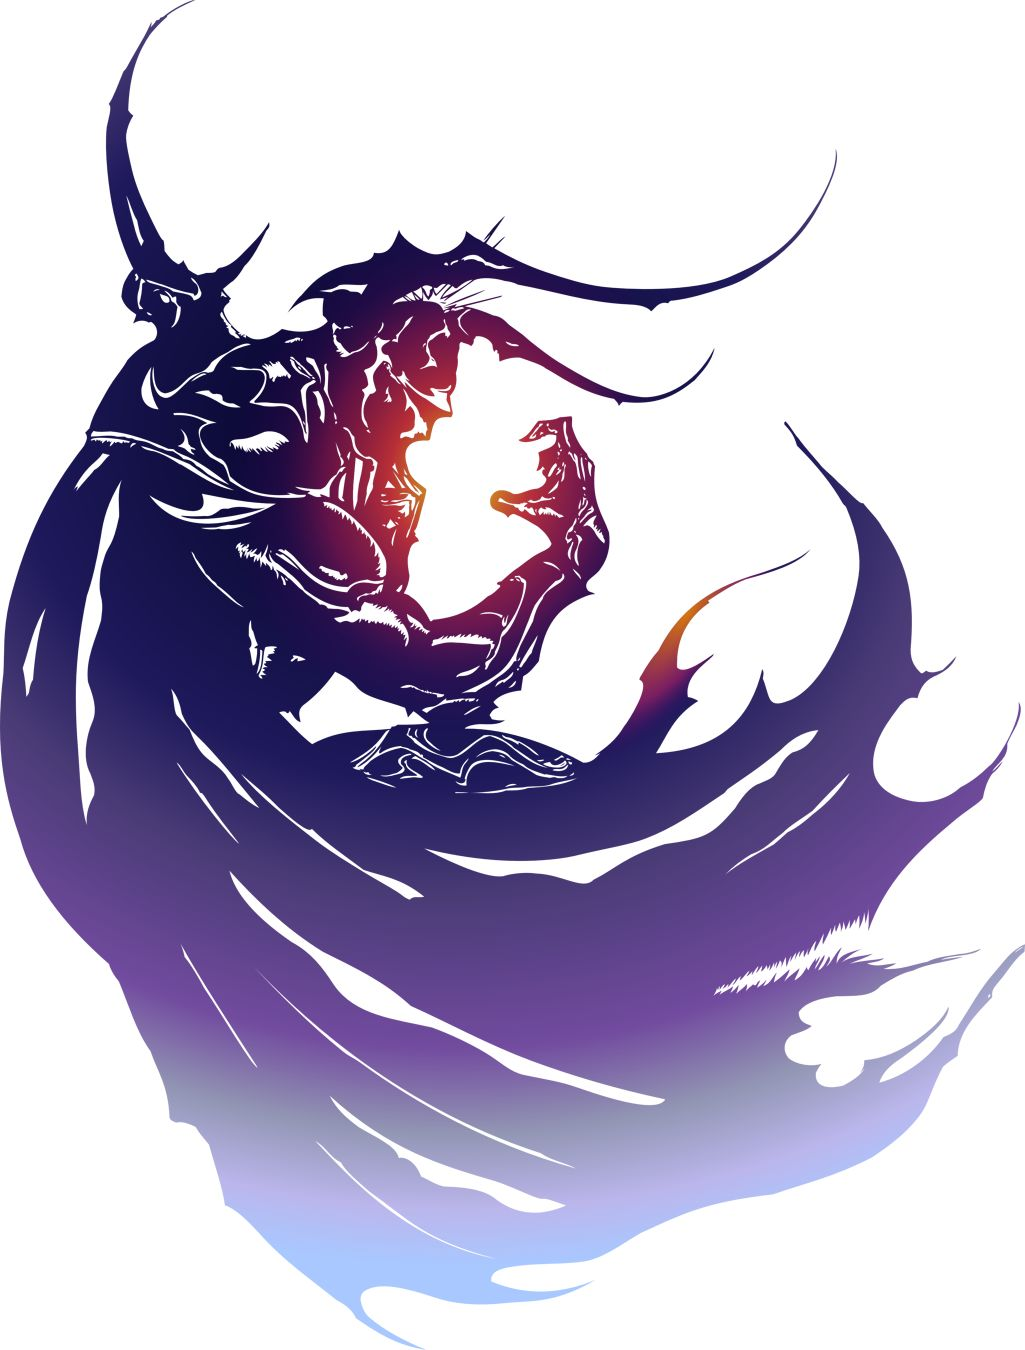
\includegraphics[width=\columnwidth]{./art/images/ff4.jpg} \\
%
\vfill
%
The \accf{Game Master} has a different role compared to the players, who play from the perspective of the protagonists.
He creates the world and setting of the adventure and takes the role of all non-player characters.
Furthermore, the GM describes the environment and narrates the outcomes of all actions. 
Unlike the players, the GM is not bound by strict rules and may make his own rulings when necessary.
This chapter can be separated into two major sections: the following short one discusses general guidelines on the various tasks of a GM, such as world creation and handling of social and combat encounters.
The second section of this chapter is a large collection of optional and modular supplements to the game, including pre-prepared content and specialized rule sets.
%
\vfill
%
Most adventures are too long to be completed in a single sitting and have to be divided into multiple \accf{sessions}.
Therefore, it is sufficient to prepare content only for the next session instead of everything in advance.
Often, it also makes sense to dedicate the very first session of an adventure on its setup, including an introduction of the setting and the player characters.
During gameplay, look out for opportunities to gracefully end an ongoing session, for example after the conclusion of a quest.
Sessions can be planned according to adventure Milestones, where Level ups should occur roughly every one to four sessions.
Still, you will not be able to prepare for everything, so do not be afraid to improvise when necessary.
%
\newpage
%
\accf{Checks} are a powerful tool that help you to decide the outcome of uncertain actions.
When players attempt actions you can ask them for checks by assigning a secret DC to the task.
In some situations you can also proactively ask players to make checks, for example to decide whether the party notices an ambush.
All non-player characters controlled by you may also have to do checks, as they follow the same rules.
However, you can refrain from using checks whenever the outcome of an action is reasonably clear.
Also note that you have two tools to modify checks: \accf{(Dis)advantage} and \accf{Fortune Dice}. 
Giving Advantage on a check allows you to express that the odds are unusually in the favor of the actor, for example because he is very well prepared or has help from another character. 
In contrast, Disadvantage usually implies that something is actively working against him, which could be a natural circumstance but also a particularly clumsy or unsuitable approach to the problem by the actor.
In comparison, Fortune Dice allow the party to benefit from random luck in some situations, but suffer from misfortune in others.
While players can use them to improve their odds in crucial moments, you can use them to create dramatic and unexpected moments.
For example, while the party is running away from their pursuers, they perform a check to avoid an obstacle on the ground and you can use a low Fortune Die to make sure that a characters trips. 
Will the rest of the party help their friend and be confronted with the pursuers or will they leave him behind and return to save him later?
%
\ofpar
%
\ofboxwithtitle{Example: Using Checks}{
	Zidane and Blank try to deliver a convincing staged sword fight to an audience of nobles.
	The GM decides that this is difficult (DC 9), because the nobles have high expectations. 
	Zidane rolls 2d with the result 9, so he barely passes the check. 
	The GM decides that most of the nobles are happy with the delivered performance, but Queen Brahme is not impressed. 
}
%
\ofpar
%
The players can get familiar with the world, by \accf{exploring} different locations.
However, travelling on foot is often not the best choice due to difficult terrain, weather or ambushes.
Depending on the setting, more comfortable forms of transportation might be available such as ships, trains, airships, cars or Chocobos.
Usually, the party needs to employ such a service, but as they become more wealthy, they may acquire their own vehicles.
For longer journeys, keep track of the amount of time that passes, which also affects the rest of the world.
\accf{Time} often passes at a different speed in the game than at your table, because uneventful aspects of the adventure can be narrated quickly, while important decisions need to be thought through more carefully.
To immerse yourself and the players into your world, it is also helpful to give short, vivid descriptions of the party's current surroundings.
In doing so, focus on elements that could be interesting for the players to interact with.
Likewise, picture the descriptions given by players about their character's actions to create your narrations of the outcome.
This often requires you to take the role of many different characters yourself to interact with the party.
In that case, understand the perspective of the character to portray how they would talk and act when confronted with the party.
%
\ofpar
%
\ofboxwithtitle{Example: Narrating \& Roleplaying\vspace*{0.2cm}}
{
	\acc{Yasumi (Game Master):}
	As you enter Riovannes Castle, you find yourself inside a large hall with narrow water streams running on both sides.
	Among multiple dead knights that lie scattered on the ground, you can see a man standing at the end of the central stairway.
	He turns around and you realize it is none other than Wiegraf Folles! \vspace{0.25cm}\\
	\acc{Yasumi (playing as Wiegraf):} There you are Ramza. Draw your sword. \vspace{0.25cm}\\			
	\acc{Akihiko:} I don't draw my sword yet. Maybe we can solve this peacefully. \vspace{0.25cm}\\	
	\acc{Yasumi (playing as Wiegraf):} What's wrong? If you don't, I will. \vspace{0.25cm}\\			
	\acc{Akihiko (playing as Ramza):} How miserable you are. Giving away your spirit just to avenge yourself. \vspace{0.25cm}\\
	\acc{Yasumi (playing as Wiegraf):} Revenge? That's not what I'm after.
	I want to bring chaos into the world... But, don't worry. I'll kill you myself! \vspace{0.25cm}\\			
	\acc{Akihiko:} OK, NOW I definitely draw my sword! \vspace{0.25cm}\\
	\acc{Yasumi:} Alright, you can take the first turn.
}
%
\ofpar
%
To keep the game balanced and challenging, keep an eye on the \accf{Wealth} of the party, ensuring that they are rewarded fairly.
A party without sufficient Gil will not be able to afford essential items and equipment, but one with too much money may be able to avoid too many consequences.
The table below gives a rough guideline for combat rewards.
Note that rewards do not have be directly in Gil, but can also be equipment, items or materials of similar value and by default they are divided between all party members.
Aside from combat, the party can also receive rewards for completing quests, but in comparison the amount may vary greatly.
As a rule-of-thumb we recommend to hand out between one and three times the amount as for a combat encounter depending on the length and difficulty of the quest.
Another important aspect that affects the party's bottom line is the trade of goods and services.
By interacting with various traders and shopkeepers, the party can buy powerful items and equipment or sell loot to increase their wealth.
You can allow yourself and the players to negotiate, for example a merchant selling her goods in a remote and dangerous location might ask for a higher price than a village store.
Furthermore, rarely any trader will be willing to pay more than half the original value of an item to stay profitable.
A similar approach can be taken with services, where especially the price of resting in Inns or Tents has great impact on the overall difficulty of the game.
%
\\\\
%
\oftable{p{0.3\columnwidth} p{0.7\columnwidth}}
{\accf{Level} & \accf{Combat Reward per Player}}
{
	1 & 200G \ofrow
	2 & 300G \ofrow
	3 & 500G \ofrow
	4 & 800G \ofrow
	5 & 1000G \ofrow
	6 & 1200G \ofrow
	7 & 1500G \ofrow
	8 & 2000G \ofrow
	9 & 2500G \ofrow
	10 & 3000G \ofrow
}
%
\vfill
%
Although adventurers spend most of their time on the road, they may sometimes rest for extended periods in towns and villages.
During this \accf{Downtime}, characters may, aside from resting, pursue a number of side activities.
You do not need to play this out in detail, instead you can quickly narrate downtime portions.
Usually, it is sufficient to assign a cost and a time frame to the activities, but for particularly difficult tasks you can also ask the player for a check to decide whether he can successfully complete it.
The list below gives some generic examples of such downtime activities and their approximate costs and durations.
%
\\\\
%
\oftable{p{0.6\columnwidth} r r}
{\accf{Downtime Activity} & \accf{Cost} & \accf{Time}}
{
	Build a small house & 5000G & weeks \ofrow
	Build a boat or carriage & 1500G & \ofrow
	Learn a simple skill (e.g. cooking or sewing) & 250G & a week \ofrow
	Help locals with simple tasks (e.g. harvest) & 0G & a week \ofrow
	Send a letter or messenger & 100G & a day \ofrow
	Attend a local festivity & 50G & a day \ofrow
	Build a platonic relationship & 10G & a week \ofrow
	Conduct research (e.g. on a location or person) & 100G & days \ofrow
	Craft a simple tool or gadget (e.g. an axe or watch) & 200G & days \ofrow
	Explore the local area & 0G & a day \ofrow
	Write a book & 100G & weeks \ofrow
}
%
\clearpage
%
\ofquote{"World very simple place. World only have two things: things you can eat and things you no can eat."\\}{Quina}\\
%
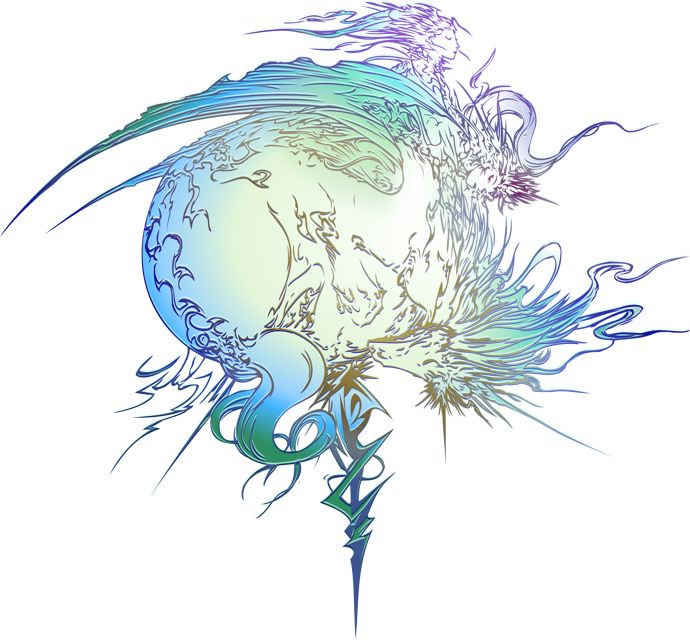
\includegraphics[width=\columnwidth]{./art/images/ff13.jpg}
%
\\\\
%
Creating a \accf{World} is one of the most difficult, but also most rewarding parts of being a GM.
The players become part of your world, where they interact with the environment and change it through their actions and decisions. 
Therefore, you can catch their interest by offering engaging content that allows for meaningful choices.
Most adventures revolve around a \accf{Central Conflict}, which the party aims to solve as the goal of their adventure.
Usually, this conflict involves multiple forces with opposing interests and the adventurers can be part of either of these sides.
Accordingly, there is also an opposing side, a common enemy or antagonist that acts against the party.
As the GM, you take the role of characters on different sides of this conflict, so you need to consider their different perspectives. 
%
\ofpar
%
A good way to start building an adventure is to establish what the world looks like on a \accf{Map}. 
Begin by creating its natural layout including landmasses, water, forests, mountains and deserts. 
Afterwards, place and mark locations that could be interesting for players to visit, like cities, dungeons or ruins.
Then add more detail only to the places that the players will likely visit in the beginning, you can do the rest later on.
You may provide the players with this map at some point in the game to make them aware of these locations you have created.
After creating some detailed locations, think about who might live in these places.
These \accf{Non-Player Characters} are roleplayed by you when interacting with the party.
They live their own lives, independent of the players and have their own personalities, goals, abilities and outlooks on life. 
Accordingly, they often have knowledge about the world that the players do not.
They can be allied, neutral or enemies of the party depending on the circumstances.
For creating detailed non-player characters, you can use the standard character creation rules, but usually it is sufficient to write down some notes about them.
%
\ofpar
%
In general, the rules try to make as few assumptions as possible to allow for greater freedom in world building.
Nevertheless, some fantasy elements are deeply ingrained into the game such as \accf{Magic}, monsters and summons.
As such, think about the role they take in your world, but you can feel free to interpret them in your own way.
For magic it is important to establish its sources, for example in Final Fantasy games, crystals are often portrayed as powerful magic sources and are thus at the center of many conflicts.
The portrayal of summons can vary greatly, as they sometimes appear as god-like beings, but in other instances they are interpreted as a mortal race.
In contrast, monsters take a similar role as wild animals, but just as summons, they are usually connected to the sources of magic and thus are able to make use of its powers.
Finally, even though we assume the existence of these magical elements, we give no restrictions concerning their prevalence, so magic in your world can be pervasive and ubiquitous, but it could also be rare and alien.
%
\ofpar
%
Another important aspect that shapes your world is the progression of \accf{Technology}.
Different technologies, such as machines, vehicles and weapons can complement the magical forces in the world, but may also stand in conflict against them.
Thus, the societies of your world may prefer or rely on magic and technology to varying degrees in their daily lives.
However, the lines between these two forces can sometimes be blurry, after all, sufficiently advanced technology is indistinguishable from magic.
During their adventure, the party can make use of available technologies and might even contribute to the current state of art.
%
\ofpar
%
\ofboxwithtitle{Example: Worldbuilding}
{
	The world we create consists two parts: Pulse and Cocoon.
	Pulse is a huge uncharted planet with a vast nature that is home to various monsters.
	In contrast, Cocoon is a small planet that floats above Pulse and is inhabited by an advanced human society.
	The Cocoon citizen depend on the god-like beings for necessities such as food and electricity.
	These powerful beings are called fal'Cie and can directly or indirectly assert control over humans.
	The fal'Cie of Cocoon stand in conflict against the fal'Cie of Pulse and accordingly humans are conditioned to be hostile towards Pulse.		
	Our adventure starts on Cocoon, where an ancient Pulse fal'Cie has been discovered some days ago.
	In a radical answer, the Cocoon government orders the deportation of all humans that have been near the Pulse fal'Cie.
	Small rebellion groups form among the citizen to fight back against this so-called "Purge".
}
%
\clearpage
%
\ofquote{With each passing day, the world finds new and exciting ways to kill a man."}{Balthier}
%
\vfill
%
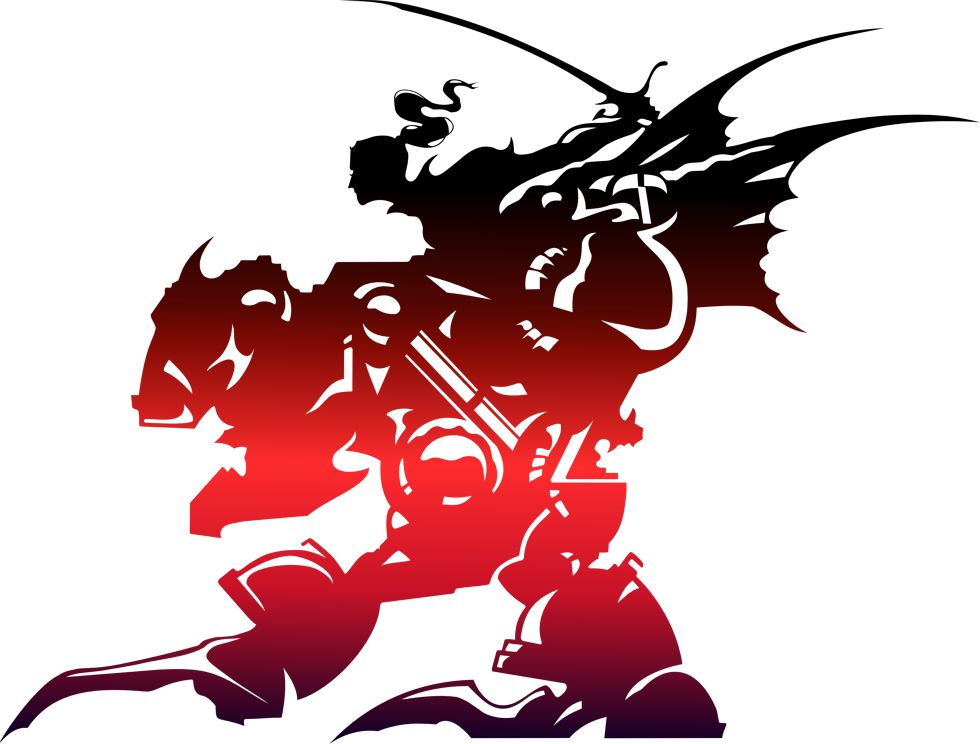
\includegraphics[width=\columnwidth]{./art/images/ff6.jpg}
%
\vfill
%
During \accf{Combat}, you play the role of all non-player characters and all regular combat rules apply to them. 
However, unlike the players, you may keep some crucial information secret, such as remaining HP and dice rolls of enemies.
While playing as an enemy party, make decisions from their perspective without using your own knowledge.
When creating combat encounters, aim to balance out the number of participants on both sides.
Large hordes of weaker enemies will often overwhelm the party, while lone ones rarely stand a chance.
A healthy mix of different enemies makes combat more interesting and balanced.
In addition, it also helpful to use visual aids like maps to keep track of the battlefield.
Combat is a matter of life and death, so it usually takes up a significant portion of playtime.
Therefore, we recommend to keep the focus on the important battles of the adventure.   
%
\vfill
%
Apart from non-player characters, \accf{Monsters} are another type of adversary that the party will often be confronted with. 
Monsters are wild beings similar to animals, that inhabit uncivilized places in the world.
Compared to animals, monsters can vary even more in their appearance and abilities due their link to magical forces.
Monsters have a natural habitat where they try to survive, so upon contact with the party they usually feel threatened and attack.
Different types of monsters often work together against hostiles, though this might not always be the case.
The party might also come across more powerful and intelligent monsters with accordingly more complex goals.
Monsters are often part or cause of ongoing conflicts and thus your adventure may feature various monsters at the center of its plot. 
In the following, we discuss the various technical aspects of creating monsters.
Note that most of these suggestions also apply for creating simple non-player character combatants. 
For important antagonist characters, we recommend to use the standard character creation rules and make additions and changes as needed.
%
\newpage
%
When creating a monster, first consider under the \accf{Circumstances} of the battle.
For example, granting a surprise round to either side can often tip the scale in an otherwise fair battle.
The composition of the player party is also crucial in determining their combat effectiveness.
A party consisting only of melee fighters will have no issues with ordinary enemies, but will likely struggle against ones with ranged damage and status effects.
In comparison, a well thought out party composition can present strategies and synergies that allow them to punch well above their weight.
In summary, understanding the strengths and weaknesses of the player party helps you to design fun and challenging encounters.
In addition, try to consider the level of experience and knowledge that the players have with the game.
Inexperienced players are prone to miss many opportunities, while very experienced ones often have unexpected tricks up their sleeves.
%
\vfill
%
You can assign the \accf{Attributes} of monsters with the following rule-of-thumb: each Level grants 6 points worth of attributes, where a point equals either 5~HP/MP or 1~STR/DEF/MAG/RES.
AGI usually ranges between 1 and 4.
Compared to characters, monsters can also vary greatly in size.
Monsters are classified as Medium~(\accf{M}) if they take up roughly 1u in diameter, as Large~(\accf{L}) if they take up more than 2u and as Small~(\accf{S}) if they take up less than 0.5u when viewed from above.
Monsters do not use regular weapons and armor, but they have equivalent parts integrated into their bodies, that follow the same rules.
Usually, we consider natural armor in the total DEF and RES and for weapons we assign the DMG of the equipment class appropriate to the monster's level.
Just like characters, monsters can also use Magic and Techniques, as well Passive and Reaction \accf{Abilities}.
However, we recommend keep the number of monster abilities low to allow for quick decisions during combat.
Still, you can feel free to give monsters access to unique and exotic abilities. 
You can also add more depth to a monster by assigning resiliences and weaknesses to specific damage types.
Note that monsters can also be inherently immune to some status effects.
During combat, you can give subtle hints about these specialties to the players when narrating combat actions and their effects.
Below is an example of a monster that was created using the guidelines discussed above.
%
\vfill
%
\ofmonster{Bomb}{3}{
\includegraphics[width=0.23\columnwidth]{./art/monsters/bomb.png}}
{
	HP: & \hfill 25 & MP: & \hfill 15\\
	STR: & \hfill 3 & DEF: & \hfill 2 \\
	MAG: & \hfill 2 & RES: & \hfill 1 \\
	AGI: & \hfill 3 & Size: & \hfill M\\
}
{\textbf{Tackle}: 1d DMG \hfill \textbf{Resilient}:\fire \hfill \textbf{Weak}:\ice }
%{}
{\mtech{Self-Destruct}{15}{1r}{2u}{Self}{Inflict KO on yourself to deal 4d fire damage to everyone within the target area.}{\fire}}
%
\clearpage
%
\accf{Gladio: "So, this Blademaster..." \ofrow Cor: "He's a master of blades. What, were you expecting something profound?"}\\\\
%
Even though we generally recommend to balance the participant count on both sides in combat, it can sometimes be interesting to have the party face very strong enemies, so-called \accf{Bosses}.
A Boss is usually significantly stronger than a player character and is either faced alone or only with some weak minions by his side.
To make up for his lack of numbers, a Boss needs not only significantly higher attributes, but also special abilities that increase his durability and allow him to take additional actions.
The table below gives some examples of such \accf{Boss Traits} that you can add to enemies you create to make them feel more like Bosses.
Note that we do not make a strict distinction between Bosses and regular enemies, but rather use the following rule-of-thumb: the more Boss Traits an enemy has, the better he can stand on his own.
%
\vfill
%
\oftable{p{0.27\columnwidth} p{0.65\columnwidth}}
{\accf{Boss Trait} & \accf{Effect}}
{
	Auto-Blink & You permanently have Blink. \ofrow
	Auto-Haste & You permanently have Haste. \ofrow
	Auto-Regen & You permanently have Regen. \ofrow
	Auto-Quicken & You can take 2 turns per round. \ofrow
	All-Immune & You have permanent Immunity against all negative Status Effects. \ofrow
	Counter & Once per round, when you suffer damage by an enemy, you can immediately make an Attack against the perpetrator if he is in range. \ofrow
	CT-0 & All of your cast times of your spells and techs are reduced to 0r.\ofrow
	Dual Attack & Whenever you perform an Attack, you can make an Attack against two different targets within range. \ofrow
	Final Attack & When you suffer KO, you may immediately take one action before falling unconscious. That action cannot prevent you from suffering KO. \ofrow
	Revert & Once per round, you may re-roll an entire die roll directly after seeing its result. \ofrow 
	Retaliate & Once per round, when you suffer damage by an enemy, you can immediately use any ability against the perpetrator if he is in its range. \ofrow
	Surge & When your current HP falls below half of its maximum, you gain EnSTR, EnDEF, EnMAG and EnRES until the end of the battle. \ofrow
}
%
\newpage
%

\ofquote{"Wait, he says... Do I look like a waiter?"\\}{Kefka}\\\\
%
The following pages are a large collection of modular \accf{Supplements} to the game.
These modules can be separated into two categories: rule changes and prepared content.
Rule changes are optional rule modifications and additions that you can use to customize your adventures.
In contrast, the prepared content provides you with optional world building blocks that you can easily incorporate in your game.
Even if you do not have a direct use for these supplements, you can still regard them as examples to create your own content.
Whenever you do use any of the given content, we strongly encourage you to make changes and additions whenever you feel it is necessary. 
Note that all of the following content is inspired by their appearance in various Final Fantasy games.
The list below gives an overview of all available supplements in the correct order with a short synopsis for each one.
%
\vfill
%
\accf{Rule Changes:}\\\\
\acc{Optional Rules:} a set of small rule changes and additions that can help you to customize the feeling of the game. \ofrow
\acc{Races:} rules and examples for incorporating different humanoid races in your game world, both for player and non-player characters.\ofrow
\acc{Chocobos:} rules for incorporating bird-like creatures called Chocobos as full-fledged party members.\ofrow
\acc{Triple Triad:} rules for a fun card game, allowing the party can collect cards and play against non-player characters.\ofrow
\acc{Blitzball:}  rules for a fun team-based sports game similar to water polo. 
%
\vfill
%
\accf{Prepared Content:}\\\\
\acc{Chaos in Cornelia:} a short adventure in which the party has to save a kidnapped princess. We highly recommend this for beginners! \ofrow
\acc{Tomb of Raithwall:} a short adventure in which the party has to recover an ancient artifact from a dangerous tomb. \ofrow
\acc{Gold Saucer:} a massive amusement park where the party can blow off steam an win rare prizes. \ofrow
\acc{Maria \& Draco:} a single-session adventure in which the party ensures the success of an opera performance. \ofrow
\acc{Siege of Dollet:} a single-session adventure in which the party has to pass a practical test to become members of an elite mercenary force. \ofrow
\acc{Worldbook:} a detailed book about the history and world of the Final Fantasy Tactics video game. \ofrow
\acc{Bestiary:} a large collection of prepared monsters.
%
\clearpage



